\section{Pianificazione}
Come riportato nelle scadenze riportate nella sottosezione 1.x, la pianificazione di progetto viene suddivisa nelle seguenti fasi:
\begin{itemize}
	\item Analisi;
	\item Consolidamento dei requisiti; (bisogna decidere se tenerla)
	\item Progettazione architetturale;
	\item Progettazione di dettaglio e codifica;
	\item Validazione e collaudo;
\end{itemize}
Ogni fase viene suddivisa in attività che verrano realizzate durante il periodo stabilito per la fase stessa.
\subsection{Analisi}
Questa fase comincia con la presentazione dei capitolati d'appalto e termina con la data di consegna per la \textit{Revisione dei Requisiti}, ovvero dal 05-11-2020 al 11-01-2021.
In questo periodo verranno redatti tutti i documenti necessari e verrà fatta un'analisi approfondita del capitolato scelto dal gruppo \Gruppo{}.

\subsubsection{Obiettivi}
Organizzazione interna del team e stesura di tutti i documenti.

\subsubsection{Periodi e attività}
La pianificazione di questa fase è stata organizzata nei seguenti periodi:
\begin{itemize}
\item \textit{Dal 05-11-2020 al 04-12-2020}: individuazione degli strumenti per la comunicazione interna e discussione dei capitolati proposti. Inizio della stesura dello \SdF{} con \glo{milestone} il 10-12-2020;

\item \textit{Dal 05-12-2020 al 22-12-2020}: stesura delle \NdP{} e del \PdP{} e iniziata inoltre la stesura dell'\AdR{}. Il 22-12-2020 il gruppo ha fissato una milestone\glo{} per la verifica dei prodotti;

\item \textit{Dal 23-12-2020 al 05-01-2021}: il gruppo si dedica all'\AdR{} e al contempo inizia la stesura del \PdQ{}. Il 05-01-2020 il gruppo fissa un'ulteriore milestone\glo{} per verificare che tutti i documenti siano stati completati correttamente;

\item \textit{Dal 06-01-2021 al 11-01-2021}: si svolge attività di verifica su tutti i documenti, si completano eventualmente documenti in ritardo. Si uniformano tutti i documenti stando alle regole stabilite nelle \NdP{}.
\end{itemize}

\begin{landscape}

\begin{figure}[h]
	\centering
	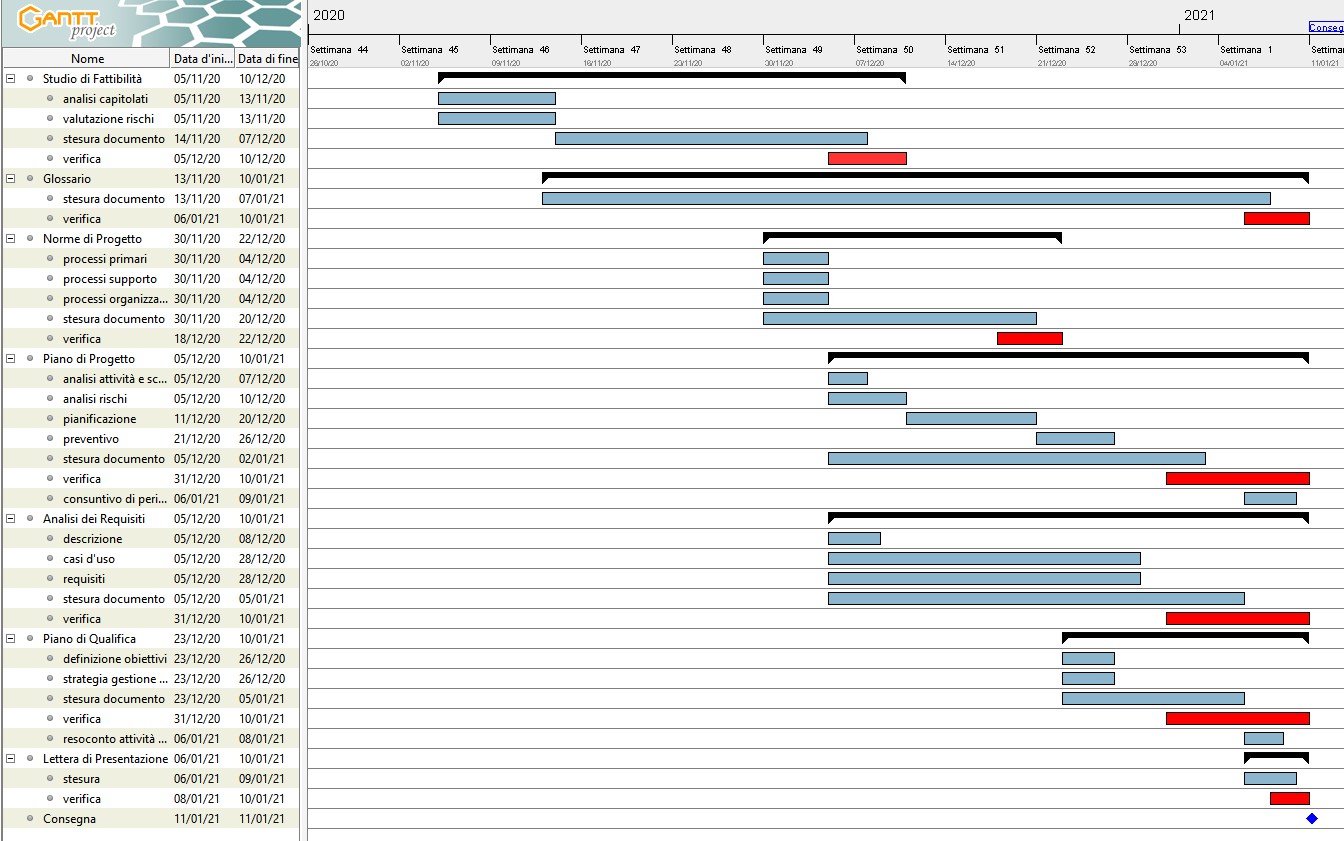
\includegraphics[width=\linewidth]{Images/GanttPianificazioneAnalisi.PNG}
	\caption{Diagramma di Gantt dell'attività di analisi}
\end{figure}

\end{landscape}




\subsection{Consolidamento}
Periodo: dal als
L'inizio del periodo di questa fase comincia con la data di formazione del gruppo e la fine coincide con la data di consegna dei documenti relativi alla revisione dei requisiti. In questa fase sono presenti le seguenti attività:
\begin{itemize}
\item attività 1
\item attività 2
\end{itemize}

GRAFICO
\subsection{Progettazione architetturale}
Questa fase comincia subito dopo la presentazione e finisce con la data di consegna per la Revisione di Progettazione, ovvero dal x/x/x all'x/x/x.\\
In questo periodo verrà individuata una soluzione architetturale che funga da sostegno per l'implementazione del prodotto. Deve soddisfare tutti i requisiti richiesti, oltre ad essere facilmente comprensibile ed attuabile. 
\begin{itemize}
\item \textbf{Incremento e verifica:} se fosse necessario, i documenti prodotti dal team verranno integrati.

 \item \glo{\textbf{Technology baseline}}: Viene fatta un'analisi ad alto livello per comprendere le tecnologie coinvolte, in due passi distinti:
\begin{itemize}
 \item \textbf{decomposizione del prodotto} in parti, in modo da essere realizzato con risorse sostenibili e costi compatibili;
 \item \textbf{analisi delle componenti individuate}, in modo da determinare come ciascuna interagisce con le altre.  
\end{itemize}
L'architettura verrà progettata sulla base di \glo{design patterns} esistenti e verrà realizzato un \glo{\textit{Proof of Concept}} da condividere con il proponente, in modo da verificare il corretto sviluppo del software. In particolare, quest'ultima attività riguarderà due incrementi:
\begin{itemize}
	\item \textbf{[codice incremento 1]}: questo periodo, che va dal x/x/x al xx(qualche giorno prima del secondo periodo in "periodi")/02/2020, ha l'obbiettivo d'implementare l'invio dei dati al \glo{back-end} con il formato richiesto. \textbf{[aggiungere riferimenti agli UC]}
	\item \textbf{[codice incremento 2]}: questo periodo, che va dal x/x/x all'xx(qualche giorno prima del secondo periodo in "periodi")/02/2020. si focalizza   sulla realizzazione dell'\glo{UI}, con la visualizzazione di un grafico di prova. \textbf{[aggiungere riferimenti agli UC]}
\end{itemize} 

\end{itemize}

\subsubsection{Periodi}
La pianificazione di questa fase è stata organizzata nel modo seguente:
\begin{itemize}
\item \textbf{18/01/2020 - xx/02/2020}: a causa della concomitanza con la sessione accademica, il team ha fissato la prima \glo{milestone} al termine di questo periodo. Alla scadenza, il gruppo dovrà aver iniziato lo studio delle tecnologie per la Technology baseline, oltre ad aver controllato buona parte della documentazione.

\item \textbf{xx/02/2020 - xx/02/2020}: per questa seconda milestone, il team s'impegnerà a terminare i lavori avviati nel periodo precedente. Inoltre l'obbiettivo è terminare il primo incremento previsto per il \textit{Proof of Concept}.

\item \textbf{xx/02/2020 - 08/03/2020}: per l'ultima milestone di questa fase, il gruppo prevede di terminare anche il secondo incremento relativo al \textit{Proof of Concept} e ultimato le verifiche.
\end{itemize}

GRAFICO
\subsection{Progettazione di dettaglio e codifica}
Questa fase comincia in seguito a quella precedente e termina con la \textit{Revisione di Qualifica}, ovvero dal 08-03-2021 al 02-04-2021. Durante questa fase verranno implementate buona parte delle componenti della web app e verranno anche aggiunte funzionalità alle componenti già sviluppate in precedenza.
Di seguito è riportato il dettaglio di ogni incremento.

\subsubsection{Incremento III}
\textit{dal 08-03-2021 al 13-03-2021}\\
L'incremento III prevede la progettazione di dettaglio e codifica delle componenti software. Si prevede di svolgere quanto segue:
\begin{itemize}
\item Implementazione di un componente per applicare una riduzione dimensionale ai dati;
\item Aggiunta di alcuni controlli per la configurazione dei parametri relativi ai diversi algoritmi di riduzione dimensionale disponibili.
\end{itemize}
\textbf{Attività}
\begin{itemize}
\item \textbf{Stesura:} eventuali correzioni ai documenti ed inizio stesura dell'allegato tecnico con scelta dei design patterns;
\item \textbf{Verifica documenti}
\item \textbf{Progettazione:} progettazione del componente per la riduzione dimensionale;
\item \textbf{Codifica:} codifica del componente per la riduzione dimensionale con relativa parametrizzazione;
\item \textbf{Verifica software:} verifica sulle funzionalità software aggiunte.
\end{itemize}
\subsubsection{Incremento IV}
\textit{dal 13-03-2021 al 17-03-2021}\\
L'incremento IV prevede la progettazione di dettaglio e codifica delle componenti software. Si prevede di svolgere quanto segue:
\begin{itemize}
\item Implementazione della visualizzazione Heat Map;
\item Aggiunta di alcuni controlli per la configurazione dei parametri relativi alla visualizzazione precedentemente implementata.
\end{itemize}
\textbf{Attività}
\begin{itemize}
\item \textbf{Stesura:} incremento della documentazione da allegare al prodotto;
\item \textbf{Verifica documenti}
\item \textbf{Progettazione:} progettazione del componente per la visualizzazione Heat Map;
\item \textbf{Codifica:} codifica del componente per la visualizzazione con relativa parametrizzazione;
\item \textbf{Verifica software:} verifica sulle funzionalità software aggiunte.
\end{itemize}

\subsubsection{Incremento V}
\textit{dal 17-03-2021 al 21-03-2021}\\
L'incremento V prevede la progettazione di dettaglio e codifica delle componenti software. Si prevede di svolgere quanto segue:
\begin{itemize}
\item Implementazione della visualizzazione Force Field;
\item Aggiunta di alcuni controlli per la configurazione dei parametri relativi alla visualizzazione precedentemente implementata.
\end{itemize}
\textbf{Attività}
\begin{itemize}
\item \textbf{Stesura:} incremento della documentazione da allegare al prodotto e inizio del manuale utente e del manuale manutentore;
\item \textbf{Verifica documenti}
\item \textbf{Progettazione:} progettazione del componente per la visualizzazione Force Field;
\item \textbf{Codifica:} codifica del componente per la visualizzazione con relativa parametrizzazione;
\item \textbf{Verifica software:} verifica sulle funzionalità software aggiunte.
\end{itemize}

\subsubsection{Incremento VI}
\textit{dal 21-03-2021 al 26-03-2021}\\
L'incremento V prevede la progettazione di dettaglio e codifica delle componenti software. Si prevede di svolgere quanto segue:
\begin{itemize}
\item Implementazione della visualizzazione Proiezione Lineare Multi Asse;
\item Aggiunta di alcuni controlli per la configurazione dei parametri relativi alla visualizzazione precedentemente implementata.
\end{itemize}
\textbf{Attività}
\begin{itemize}
\item \textbf{Stesura:} incremento della documentazione da allegare al prodotto ;
\item \textbf{Verifica documenti}
\item \textbf{Progettazione:} progettazione del componente per la visualizzazione Proiezione Lineare Multi Asse;
\item \textbf{Codifica:} codifica del componente per la visualizzazione con relativa parametrizzazione;
\item \textbf{Verifica software:} verifica sulle funzionalità software aggiunte.
\end{itemize}

\subsubsection{Incremento VII}
\textit{dal 26-03-2021 al 2-04-2021}\\
L'incremento V prevede la progettazione di dettaglio e codifica delle componenti software. Si prevede di svolgere quanto segue:
\begin{itemize}
\item Implementazione di un database;
\item Sviluppo di un componente per la scelta e il caricamento di un dataset contenuto nel database.
\end{itemize}
\textbf{Attività}
\begin{itemize}
\item \textbf{Stesura:} incremento e conclusione della documentazione da allegare al prodotto ;
\item \textbf{Verifica documenti}
\item \textbf{Progettazione:} progettazione del database e del componente per la scelta e il caricamento del dataset;
\item \textbf{Creazione struttura database:} stesura della struttura del database;
\item \textbf{Codifica:} codifica del componente per la scelta e il caricamento del dataset;
\item \textbf{Verifica software:} verifica sulle funzionalità software aggiunte.
\end{itemize}

\begin{landscape}

\begin{figure}[h]
 	\centering
	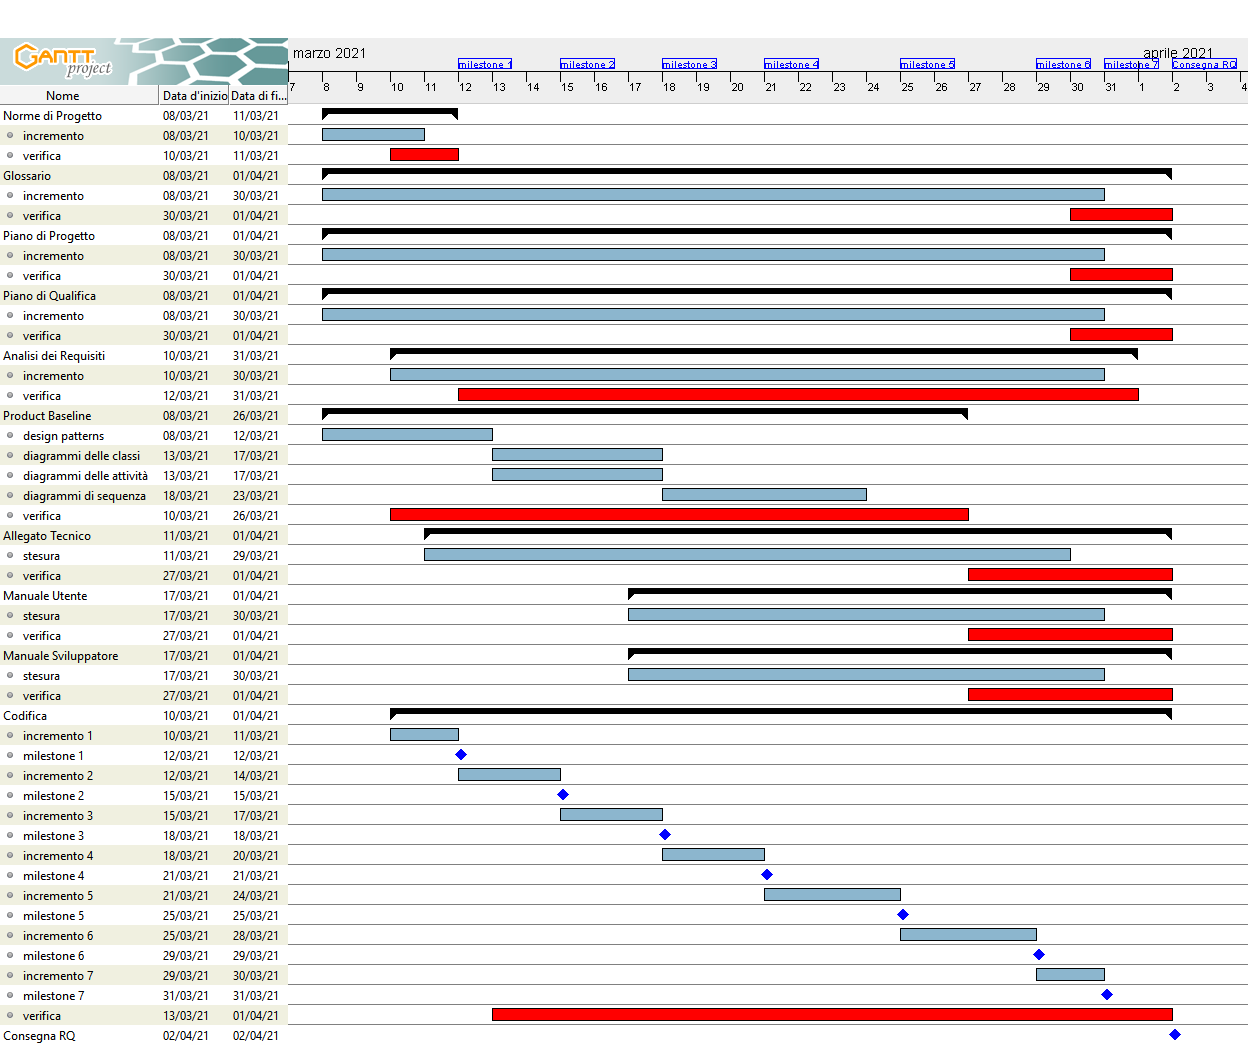
\includegraphics[width=\linewidth]{Images/GanttPianificazioneProgettazioneDettaglioCodifica.png}
	\caption{Diagramma di Gantt dell'attività di Progettazione di dettaglio e Codifica}
\end{figure}

\end{landscape}
\subsection{Validazione e Collaudo}
Questa fase comincia subito dopo la fase precedente e finisce con la data di consegna per la \textit{Revisione di Accettazione}, ovvero dal 09-04-2020 al 03-05-2020.\\
In questo periodo verranno creati ulteriori test per verificare il corretto funzionamento del prodotto. Se tutte le scadenze imposte dal gruppo vengono rispettate il tempo in eccesso viene occupato per la realizzazione di requisiti opzionali, concordati con il committente. 
\subsubsection{Attività}
\begin{itemize}
\item \textbf{Incremento e verifica dei documenti:} se fosse necessario, i documenti prodotti dal team verranno integrati.

 \item \textbf{Incremento e verifica delle attività}: sia la \textit{Technology baseline} che la \textit{Product Baseline} vengono eventualmente raffinate; particolare attenzione va alla codifica, svolta ad incrementi ciclici.
 \begin{itemize}
 \item \textbf{Incremento X}: il gruppo identifica e implementa la soluzione più adeguata per la gestione della sessione nell'applicazione. Incremento della documentazione da correlare al prodotto software e incremento della documentazione per verifica e miglioramento continuo \textbf{[UC1.2, UC7]};
\item \textbf{Incremento XI}: viene perfezionato il codice precedentemente, il prodotto viene collaudato e vengono vericati tutti i documenti precedentemente redatti. 
 \end{itemize}

 \item \textbf{Verifica e collaudo}: vengono creati e applicati un set di test, che hanno lo scopo di portare il prodotto ad un buon livello qualitativo. Il gruppo si focalizzerà sulla sua correttezza e nel rispetto di tutti i requisiti.
\end{itemize}

\subsubsection{Periodi}
La pianificazione di questa fase è stata organizzata con le seguenti milestone:

\begin{itemize}
\item \textbf{Periodo 1}: \textit{(dal 09-04-2020 al 16-04-2020)} se fosse necessario, in questo periodo viene controllata tutta la documentazione e ci si dedicherà ad eventuali incrementi della \textit{Technology Baseline} e \textit{Product Baseline}, è fissata una milestone l'ultimo giorno di questo periodo entra cui dovrà essere terminato l'incremento X.

\item \textbf{Periodo 2}: \textit{(dal 16-04-2020 al 03-05-2020)} entro la milestone del 03-05-2020 il gruppo ha come obbiettivo quello di completare l'ultimo incremento.

\end{itemize}
\newpage
\subsubsection{Diagramma di Gantt: Validazione e Collaudo}
\begin{figure}[h]
	\centering
	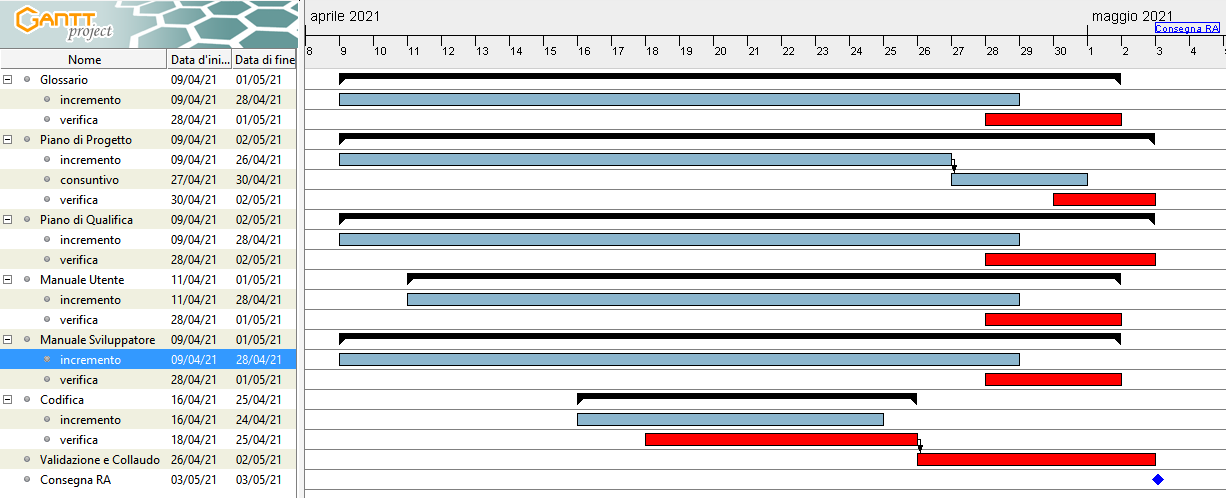
\includegraphics[scale=0.5]{Images/GanttValidazioneCollaudo.PNG}
	\caption{Diagramma di Gantt dell'attività di Validazione e Collaudo}
\end{figure}